\chapter{Analysis and Results}
\label{cap:AnalysisandResults}
In this chapter the analysis and the result of the research findings will be presented. 

\section{Traffic Capturing}
Standby traffic was captured between 8 and 22  of January. During this time period, no interaction with the vacuum cleaner was done. It was also continuously connected to WiFi, enabling Internet connectivity.

Event objectives are captured in Oslo and Drammen environments according to the test matrices \ref{tab:TestMatrixEnv1} \ref{tab:TestMatrixEnv2}. All events was observers finished, before a new event was triggered. Capturing in Drammen was done during four days, due to limited availability of the smart environment.  
\begin{table}[H]
\centering
\small
\caption{Test matrix Oslo}
\label{tab:TestMatrixEnv1}
\begin{tabular}{|lllllllllll|}
\hline
\multicolumn{11}{|c|}{\textbf{Scheduled cleaning}}                                                                                                                                                                                                                                                        \\ \hline
\multicolumn{1}{|l|}{Nr} & \multicolumn{1}{l|}{1}     & \multicolumn{1}{l|}{2}     & \multicolumn{1}{l|}{3}     & \multicolumn{1}{l|}{4}     & \multicolumn{1}{l|}{5}     & \multicolumn{1}{l|}{6}     & \multicolumn{1}{l|}{7}     & \multicolumn{1}{l|}{8}     & \multicolumn{1}{l|}{9}     & 10    \\ \hline
\multicolumn{1}{|l|}{Date}   & \multicolumn{1}{l|}{10.03} & \multicolumn{1}{l|}{10.03} & \multicolumn{1}{l|}{10.03} & \multicolumn{1}{l|}{10.03} & \multicolumn{1}{l|}{10.03} & \multicolumn{1}{l|}{10.03} & \multicolumn{1}{l|}{10.03} & \multicolumn{1}{l|}{10.03} & \multicolumn{1}{l|}{11.03} & 11.03 \\ \hline
\multicolumn{1}{|l|}{Start}  & \multicolumn{1}{l|}{10:44} & \multicolumn{1}{l|}{11:14} & \multicolumn{1}{l|}{12:14} & \multicolumn{1}{l|}{13:29} & \multicolumn{1}{l|}{14:59} & \multicolumn{1}{l|}{15:29} & \multicolumn{1}{l|}{15:54} & \multicolumn{1}{l|}{16:09} & \multicolumn{1}{l|}{10:09} & 10:29 \\ \hline
\multicolumn{1}{|l|}{End}    & \multicolumn{1}{l|}{10:54} & \multicolumn{1}{l|}{11:24} & \multicolumn{1}{l|}{12:24} & \multicolumn{1}{l|}{13:39} & \multicolumn{1}{l|}{15:09} & \multicolumn{1}{l|}{15:39} & \multicolumn{1}{l|}{16:04} & \multicolumn{1}{l|}{16:19} & \multicolumn{1}{l|}{10:19} & 10:39 \\ \hline
\multicolumn{11}{|c|}{\textbf{Application triggered cleaning}}                                                                                                                                                                                                                                            \\ \hline
\multicolumn{1}{|l|}{Nr} & \multicolumn{1}{l|}{1}     & \multicolumn{1}{l|}{2}     & \multicolumn{1}{l|}{3}     & \multicolumn{1}{l|}{4}     & \multicolumn{1}{l|}{5}     & \multicolumn{1}{l|}{6}     & \multicolumn{1}{l|}{7}     & \multicolumn{1}{l|}{8}     & \multicolumn{1}{l|}{9}     & 10    \\ \hline
\multicolumn{1}{|l|}{Date}   & \multicolumn{1}{l|}{28.02} & \multicolumn{1}{l|}{28.02} & \multicolumn{1}{l|}{01.03} & \multicolumn{1}{l|}{09.03} & \multicolumn{1}{l|}{09.03} & \multicolumn{1}{l|}{09.03} & \multicolumn{1}{l|}{09.03} & \multicolumn{1}{l|}{09.03} & \multicolumn{1}{l|}{12.03} & 12.03 \\ \hline
\multicolumn{1}{|l|}{Start}  & \multicolumn{1}{l|}{18:20} & \multicolumn{1}{l|}{18:35} & \multicolumn{1}{l|}{18:53} & \multicolumn{1}{l|}{07:44} & \multicolumn{1}{l|}{08:03} & \multicolumn{1}{l|}{08:25} & \multicolumn{1}{l|}{08:57} & \multicolumn{1}{l|}{09:18} & \multicolumn{1}{l|}{12:20} & 12:54 \\ \hline
\multicolumn{1}{|l|}{End}    & \multicolumn{1}{l|}{18:27} & \multicolumn{1}{l|}{18:42} & \multicolumn{1}{l|}{19:00} & \multicolumn{1}{l|}{07:49} & \multicolumn{1}{l|}{08:10} & \multicolumn{1}{l|}{08:31} & \multicolumn{1}{l|}{09:04} & \multicolumn{1}{l|}{09:26} & \multicolumn{1}{l|}{12:35} & 13:09 \\ \hline
\multicolumn{11}{|c|}{\textbf{Open application}}                                                                                                                                                                                                                                                          \\ \hline
\multicolumn{1}{|l|}{Nr} & \multicolumn{1}{l|}{1}     & \multicolumn{1}{l|}{2}     & \multicolumn{1}{l|}{3}     & \multicolumn{1}{l|}{4}     & \multicolumn{1}{l|}{5}     & \multicolumn{1}{l|}{6}     & \multicolumn{1}{l|}{7}     & \multicolumn{1}{l|}{8}     & \multicolumn{1}{l|}{9}     & 10    \\ \hline
\multicolumn{1}{|l|}{Date}   & \multicolumn{1}{l|}{10.03} & \multicolumn{1}{l|}{10.03} & \multicolumn{1}{l|}{10.03} & \multicolumn{1}{l|}{10.03} & \multicolumn{1}{l|}{10.03} & \multicolumn{1}{l|}{10.03} & \multicolumn{1}{l|}{10.03} & \multicolumn{1}{l|}{10.03} & \multicolumn{1}{l|}{11.03} & 11.03 \\ \hline
\multicolumn{1}{|l|}{Start}  & \multicolumn{1}{l|}{10:26} & \multicolumn{1}{l|}{11:06} & \multicolumn{1}{l|}{11:56} & \multicolumn{1}{l|}{13:22} & \multicolumn{1}{l|}{14:58} & \multicolumn{1}{l|}{15:27} & \multicolumn{1}{l|}{15:51} & \multicolumn{1}{l|}{16:07} & \multicolumn{1}{l|}{10:06} & 10:22 \\ \hline
\multicolumn{1}{|l|}{End}    & \multicolumn{1}{l|}{10:36} & \multicolumn{1}{l|}{11:16} & \multicolumn{1}{l|}{12:06} & \multicolumn{1}{l|}{13:32} & \multicolumn{1}{l|}{15:08} & \multicolumn{1}{l|}{15:37} & \multicolumn{1}{l|}{16:01} & \multicolumn{1}{l|}{16:17} & \multicolumn{1}{l|}{10:16} & 10:32 \\ \hline
\multicolumn{11}{|c|}{\textbf{Remove bin}}                                                                                                                                                                                                                                                                \\ \hline
\multicolumn{1}{|l|}{Nr} & \multicolumn{1}{l|}{1}     & \multicolumn{1}{l|}{2}     & \multicolumn{1}{l|}{3}     & \multicolumn{1}{l|}{4}     & \multicolumn{1}{l|}{5}     & \multicolumn{1}{l|}{6}     & \multicolumn{1}{l|}{7}     & \multicolumn{1}{l|}{8}     & \multicolumn{1}{l|}{9}     & 10    \\ \hline
\multicolumn{1}{|l|}{Date}   & \multicolumn{1}{l|}{11.03} & \multicolumn{1}{l|}{11.03} & \multicolumn{1}{l|}{11.03} & \multicolumn{1}{l|}{11.03} & \multicolumn{1}{l|}{11.03} & \multicolumn{1}{l|}{11.03} & \multicolumn{1}{l|}{11.03} & \multicolumn{1}{l|}{11.03} & \multicolumn{1}{l|}{11.03} & 11.03 \\ \hline
\multicolumn{1}{|l|}{Start}  & \multicolumn{1}{l|}{17:30} & \multicolumn{1}{l|}{17:35} & \multicolumn{1}{l|}{17:40} & \multicolumn{1}{l|}{17:44} & \multicolumn{1}{l|}{17:47} & \multicolumn{1}{l|}{17:49} & \multicolumn{1}{l|}{17:51} & \multicolumn{1}{l|}{17:53} & \multicolumn{1}{l|}{17:55} & 18:01 \\ \hline
\multicolumn{1}{|l|}{End}    & \multicolumn{1}{l|}{17:31} & \multicolumn{1}{l|}{17:36} & \multicolumn{1}{l|}{17:41} & \multicolumn{1}{l|}{17:45} & \multicolumn{1}{l|}{17:48} & \multicolumn{1}{l|}{17:50} & \multicolumn{1}{l|}{17:52} & \multicolumn{1}{l|}{17:54} & \multicolumn{1}{l|}{17:56} & 18:02 \\ \hline
\multicolumn{11}{|c|}{\textbf{Physical triggered cleaning}}                                                                                                                                                                                                                                               \\ \hline
\multicolumn{1}{|l|}{Nr} & \multicolumn{1}{l|}{1}     & \multicolumn{1}{l|}{2}     & \multicolumn{1}{l|}{3}     & \multicolumn{1}{l|}{4}     & \multicolumn{1}{l|}{5}     & \multicolumn{1}{l|}{6}     & \multicolumn{1}{l|}{7}     & \multicolumn{1}{l|}{8}     & \multicolumn{1}{l|}{9}     & 10    \\ \hline
\multicolumn{1}{|l|}{Date}   & \multicolumn{1}{l|}{23.02} & \multicolumn{1}{l|}{23.02} & \multicolumn{1}{l|}{23.02} & \multicolumn{1}{l|}{23.02} & \multicolumn{1}{l|}{23.02} & \multicolumn{1}{l|}{09.03} & \multicolumn{1}{l|}{09.03} & \multicolumn{1}{l|}{09.03} & \multicolumn{1}{l|}{09.03} & 09.03 \\ \hline
\multicolumn{1}{|l|}{Start}  & \multicolumn{1}{l|}{18:08} & \multicolumn{1}{l|}{18:36} & \multicolumn{1}{l|}{19:14} & \multicolumn{1}{l|}{20:13} & \multicolumn{1}{l|}{20:44} & \multicolumn{1}{l|}{09:43} & \multicolumn{1}{l|}{10:30} & \multicolumn{1}{l|}{12:32} & \multicolumn{1}{l|}{13:16} & 17:44 \\ \hline
\multicolumn{1}{|l|}{End}    & \multicolumn{1}{l|}{18:24} & \multicolumn{1}{l|}{19:05} & \multicolumn{1}{l|}{19:34} & \multicolumn{1}{l|}{20:35} & \multicolumn{1}{l|}{21:06} & \multicolumn{1}{l|}{10:02} & \multicolumn{1}{l|}{10:50} & \multicolumn{1}{l|}{12:50} & \multicolumn{1}{l|}{14:05} & 18:05 \\ \hline
\multicolumn{11}{|c|}{\textbf{Automated cleaning}}                                                                                                                                                                                                                                                        \\ \hline
\multicolumn{1}{|l|}{Nr} & \multicolumn{1}{l|}{1}     & \multicolumn{1}{l|}{2}     & \multicolumn{1}{l|}{3}     & \multicolumn{1}{l|}{4}     & \multicolumn{1}{l|}{5}     & \multicolumn{1}{l|}{6}     & \multicolumn{1}{l|}{7}     & \multicolumn{1}{l|}{8}     & \multicolumn{1}{l|}{9}     & 10    \\ \hline
\multicolumn{1}{|l|}{Date}   & \multicolumn{1}{l|}{21.02} & \multicolumn{1}{l|}{22.02} & \multicolumn{1}{l|}{23.02} & \multicolumn{1}{l|}{01.03} & \multicolumn{1}{l|}{02.03} & \multicolumn{1}{l|}{03.03} & \multicolumn{1}{l|}{06.03} & \multicolumn{1}{l|}{07.03} & \multicolumn{1}{l|}{08.03} & 09.03 \\ \hline
\multicolumn{1}{|l|}{Start}  & \multicolumn{1}{l|}{21:06} & \multicolumn{1}{l|}{07:37} & \multicolumn{1}{l|}{10:10} & \multicolumn{1}{l|}{07:42} & \multicolumn{1}{l|}{11:05} & \multicolumn{1}{l|}{07:03} & \multicolumn{1}{l|}{07:04} & \multicolumn{1}{l|}{08:42} & \multicolumn{1}{l|}{07:49} & 07:22 \\ \hline
\multicolumn{1}{|l|}{End}    & \multicolumn{1}{l|}{21:14} & \multicolumn{1}{l|}{07:45} & \multicolumn{1}{l|}{10:16} & \multicolumn{1}{l|}{07:47} & \multicolumn{1}{l|}{11:10} & \multicolumn{1}{l|}{07:08} & \multicolumn{1}{l|}{07:09} & \multicolumn{1}{l|}{08:47} & \multicolumn{1}{l|}{07:54} & 07:29 \\ \hline
\end{tabular}
\end{table}


\begin{table}[H]
\small
\centering
\caption{Test matrix Drammen}
\label{tab:TestMatrixEnv2}
\begin{tabular}{|lllllllllll|}
\hline
\multicolumn{11}{|c|}{\textbf{Scheduled cleaning}}                                                                                                                                                                                                                                                        \\ \hline
\multicolumn{1}{|l|}{Nr} & \multicolumn{1}{l|}{1}     & \multicolumn{1}{l|}{2}     & \multicolumn{1}{l|}{3}     & \multicolumn{1}{l|}{4}     & \multicolumn{1}{l|}{5}     & \multicolumn{1}{l|}{6}     & \multicolumn{1}{l|}{7}     & \multicolumn{1}{l|}{8}     & \multicolumn{1}{l|}{9}     & 10    \\ \hline
\multicolumn{1}{|l|}{Date}   & \multicolumn{1}{l|}{25.02} & \multicolumn{1}{l|}{25.02} & \multicolumn{1}{l|}{26.02} & \multicolumn{1}{l|}{26.02} & \multicolumn{1}{l|}{26.02} & \multicolumn{1}{l|}{26.02} & \multicolumn{1}{l|}{26.02} & \multicolumn{1}{l|}{26.02} & \multicolumn{1}{l|}{26.02} & 26.02 \\ \hline
\multicolumn{1}{|l|}{Start}  & \multicolumn{1}{l|}{20:30} & \multicolumn{1}{l|}{21:00} & \multicolumn{1}{l|}{11:20} & \multicolumn{1}{l|}{11:50} & \multicolumn{1}{l|}{12:20} & \multicolumn{1}{l|}{12:50} & \multicolumn{1}{l|}{13:20} & \multicolumn{1}{l|}{13:50} & \multicolumn{1}{l|}{14:20} & 15:00 \\ \hline
\multicolumn{1}{|l|}{End}    & \multicolumn{1}{l|}{20:45} & \multicolumn{1}{l|}{21:15} & \multicolumn{1}{l|}{11:35} & \multicolumn{1}{l|}{12:05} & \multicolumn{1}{l|}{12:35} & \multicolumn{1}{l|}{13:05} & \multicolumn{1}{l|}{13:35} & \multicolumn{1}{l|}{14:05} & \multicolumn{1}{l|}{14:35} & 15:15 \\ \hline
\multicolumn{11}{|c|}{\textbf{Application triggered cleaning}}                                                                                                                                                                                                                                            \\ \hline
\multicolumn{1}{|l|}{Nr} & \multicolumn{1}{l|}{1}     & \multicolumn{1}{l|}{2}     & \multicolumn{1}{l|}{3}     & \multicolumn{1}{l|}{4}     & \multicolumn{1}{l|}{5}     & \multicolumn{1}{l|}{6}     & \multicolumn{1}{l|}{7}     & \multicolumn{1}{l|}{8}     & \multicolumn{1}{l|}{9}     & 10    \\ \hline
\multicolumn{1}{|l|}{Date}   & \multicolumn{1}{l|}{25.02} & \multicolumn{1}{l|}{25.02} & \multicolumn{1}{l|}{25.02} & \multicolumn{1}{l|}{25.02} & \multicolumn{1}{l|}{25.02} & \multicolumn{1}{l|}{25.02} & \multicolumn{1}{l|}{25.02} & \multicolumn{1}{l|}{25.02} & \multicolumn{1}{l|}{25.02} & 25.02 \\ \hline
\multicolumn{1}{|l|}{Start}  & \multicolumn{1}{l|}{14:30} & \multicolumn{1}{l|}{15:00} & \multicolumn{1}{l|}{15:30} & \multicolumn{1}{l|}{16:00} & \multicolumn{1}{l|}{16:30} & \multicolumn{1}{l|}{17:00} & \multicolumn{1}{l|}{17:30} & \multicolumn{1}{l|}{19:00} & \multicolumn{1}{l|}{19:30} & 20:00 \\ \hline
\multicolumn{1}{|l|}{End}    & \multicolumn{1}{l|}{14:45} & \multicolumn{1}{l|}{15:15} & \multicolumn{1}{l|}{15:45} & \multicolumn{1}{l|}{16:15} & \multicolumn{1}{l|}{16:45} & \multicolumn{1}{l|}{17:15} & \multicolumn{1}{l|}{17:45} & \multicolumn{1}{l|}{19:15} & \multicolumn{1}{l|}{19:45} & 20:15 \\ \hline
\multicolumn{11}{|c|}{\textbf{Open application}}                                                                                                                                                                                                                                                          \\ \hline
\multicolumn{1}{|l|}{Nr} & \multicolumn{1}{l|}{1}     & \multicolumn{1}{l|}{2}     & \multicolumn{1}{l|}{3}     & \multicolumn{1}{l|}{4}     & \multicolumn{1}{l|}{5}     & \multicolumn{1}{l|}{6}     & \multicolumn{1}{l|}{7}     & \multicolumn{1}{l|}{8}     & \multicolumn{1}{l|}{9}     & 10    \\ \hline
\multicolumn{1}{|l|}{Date}   & \multicolumn{1}{l|}{25.02} & \multicolumn{1}{l|}{25.02} & \multicolumn{1}{l|}{25.02} & \multicolumn{1}{l|}{25.02} & \multicolumn{1}{l|}{26.02} & \multicolumn{1}{l|}{26.02} & \multicolumn{1}{l|}{26.02} & \multicolumn{1}{l|}{26.02} & \multicolumn{1}{l|}{26.02} & 26.02 \\ \hline
\multicolumn{1}{|l|}{Start}  & \multicolumn{1}{l|}{20:50} & \multicolumn{1}{l|}{21:20} & \multicolumn{1}{l|}{22:20} & \multicolumn{1}{l|}{22:50} & \multicolumn{1}{l|}{11:10} & \multicolumn{1}{l|}{11:40} & \multicolumn{1}{l|}{12:10} & \multicolumn{1}{l|}{12:40} & \multicolumn{1}{l|}{13:10} & 13:40 \\ \hline
\multicolumn{1}{|l|}{End}    & \multicolumn{1}{l|}{20:52} & \multicolumn{1}{l|}{21:21} & \multicolumn{1}{l|}{22:22} & \multicolumn{1}{l|}{22:52} & \multicolumn{1}{l|}{11:11} & \multicolumn{1}{l|}{11:41} & \multicolumn{1}{l|}{12:11} & \multicolumn{1}{l|}{12:41} & \multicolumn{1}{l|}{13:11} & 13:41 \\ \hline
\multicolumn{11}{|c|}{\textbf{Remove bin}}                                                                                                                                                                                                                                                                \\ \hline
\multicolumn{1}{|l|}{Nr} & \multicolumn{1}{l|}{1}     & \multicolumn{1}{l|}{2}     & \multicolumn{1}{l|}{3}     & \multicolumn{1}{l|}{4}     & \multicolumn{1}{l|}{5}     & \multicolumn{1}{l|}{6}     & \multicolumn{1}{l|}{7}     & \multicolumn{1}{l|}{8}     & \multicolumn{1}{l|}{9}     & 10    \\ \hline
\multicolumn{1}{|l|}{Date}   & \multicolumn{1}{l|}{26.02} & \multicolumn{1}{l|}{26.02} & \multicolumn{1}{l|}{26.02} & \multicolumn{1}{l|}{27.02} & \multicolumn{1}{l|}{27.02} & \multicolumn{1}{l|}{27.02} & \multicolumn{1}{l|}{27.02} & \multicolumn{1}{l|}{27.02} & \multicolumn{1}{l|}{27.02} & 27.02 \\ \hline
\multicolumn{1}{|l|}{Start}  & \multicolumn{1}{l|}{15:22} & \multicolumn{1}{l|}{15:30} & \multicolumn{1}{l|}{15:35} & \multicolumn{1}{l|}{15:05} & \multicolumn{1}{l|}{15:10} & \multicolumn{1}{l|}{15:15} & \multicolumn{1}{l|}{15:20} & \multicolumn{1}{l|}{15:25} & \multicolumn{1}{l|}{15:30} & 15:35 \\ \hline
\multicolumn{1}{|l|}{End}    & \multicolumn{1}{l|}{15:23} & \multicolumn{1}{l|}{15:31} & \multicolumn{1}{l|}{15:36} & \multicolumn{1}{l|}{15:06} & \multicolumn{1}{l|}{15:11} & \multicolumn{1}{l|}{15:16} & \multicolumn{1}{l|}{15:21} & \multicolumn{1}{l|}{15:26} & \multicolumn{1}{l|}{15:31} & 15:36 \\ \hline
\multicolumn{11}{|c|}{\textbf{Physical triggered cleaning}}                                                                                                                                                                                                                                               \\ \hline
\multicolumn{1}{|l|}{Nr} & \multicolumn{1}{l|}{1}     & \multicolumn{1}{l|}{2}     & \multicolumn{1}{l|}{3}     & \multicolumn{1}{l|}{4}     & \multicolumn{1}{l|}{5}     & \multicolumn{1}{l|}{6}     & \multicolumn{1}{l|}{7}     & \multicolumn{1}{l|}{8}     & \multicolumn{1}{l|}{9}     & 10    \\ \hline
\multicolumn{1}{|l|}{Date}   & \multicolumn{1}{l|}{25.02} & \multicolumn{1}{l|}{25.02} & \multicolumn{1}{l|}{25.02} & \multicolumn{1}{l|}{25.02} & \multicolumn{1}{l|}{25.02} & \multicolumn{1}{l|}{26.02} & \multicolumn{1}{l|}{26.02} & \multicolumn{1}{l|}{26.02} & \multicolumn{1}{l|}{26.02} & 26.02 \\ \hline
\multicolumn{1}{|l|}{Start}  & \multicolumn{1}{l|}{22:00} & \multicolumn{1}{l|}{22:30} & \multicolumn{1}{l|}{23:00} & \multicolumn{1}{l|}{23:20} & \multicolumn{1}{l|}{23:40} & \multicolumn{1}{l|}{00:00} & \multicolumn{1}{l|}{00:20} & \multicolumn{1}{l|}{00:40} & \multicolumn{1}{l|}{01:06} & 01:31 \\ \hline
\multicolumn{1}{|l|}{End}    & \multicolumn{1}{l|}{22:12} & \multicolumn{1}{l|}{22:45} & \multicolumn{1}{l|}{23:15} & \multicolumn{1}{l|}{23:35} & \multicolumn{1}{l|}{23:55} & \multicolumn{1}{l|}{00:15} & \multicolumn{1}{l|}{00:35} & \multicolumn{1}{l|}{00:55} & \multicolumn{1}{l|}{01:20} & 01:45 \\ \hline
\multicolumn{11}{|c|}{\textbf{Automated cleaning}}                                                                                                                                                                                                                                                        \\ \hline
\multicolumn{1}{|l|}{Nr} & \multicolumn{1}{l|}{1}     & \multicolumn{1}{l|}{2}     & \multicolumn{1}{l|}{3}     & \multicolumn{1}{l|}{4}     & \multicolumn{1}{l|}{5}     & \multicolumn{1}{l|}{6}     & \multicolumn{1}{l|}{7}     & \multicolumn{1}{l|}{8}     & \multicolumn{1}{l|}{9}     & 10    \\ \hline
\multicolumn{1}{|l|}{Date}   & \multicolumn{1}{l|}{25.02} & \multicolumn{1}{l|}{26.02} & \multicolumn{1}{l|}{26.02} & \multicolumn{1}{l|}{26.02} & \multicolumn{1}{l|}{26.02} & \multicolumn{1}{l|}{27.02} & \multicolumn{1}{l|}{27.02} & \multicolumn{1}{l|}{27.02} & \multicolumn{1}{l|}{27.02} & 27.02 \\ \hline
\multicolumn{1}{|l|}{Start}  & \multicolumn{1}{l|}{21:32} & \multicolumn{1}{l|}{01:53} & \multicolumn{1}{l|}{15:43} & \multicolumn{1}{l|}{17:00} & \multicolumn{1}{l|}{22:11} & \multicolumn{1}{l|}{07:57} & \multicolumn{1}{l|}{08:51} & \multicolumn{1}{l|}{11:03} & \multicolumn{1}{l|}{12:04} & 13:36 \\ \hline
\multicolumn{1}{|l|}{End}    & \multicolumn{1}{l|}{21:50} & \multicolumn{1}{l|}{02:10} & \multicolumn{1}{l|}{15:55} & \multicolumn{1}{l|}{17:12} & \multicolumn{1}{l|}{22:23} & \multicolumn{1}{l|}{08:10} & \multicolumn{1}{l|}{09:02} & \multicolumn{1}{l|}{11:13} & \multicolumn{1}{l|}{12:16} & 13:48 \\ \hline
\end{tabular}
\end{table}

During the traffic capturing and event triggering, we did some interesting observations. Whenever changes was done to schedule cleaning configuration through the application, the robot vacuum cleaner made a sound. The configuration is probably saved and sent to the vacuum cleaner right a way. Another observation on the scheduled cleaning events was that, the robot vacuum cleaner always started cleaning within 1 minutes before the clean was actually configures. If the cleaning was scheduled 08:00, it would start between 07:59:30 and 07:59:50.

During physical cleaning the robot vacuum cleaner several times though it had been placed in a new floor or room and started doing smart floor detection. The duration of this discovery process is mush more time consuming than the actual cleaning. This is probably the reason why physical triggered cleaning event, 2 and 9 in Oslo, was significantly longer then the average.
During the Application start event it looks like the application are pulling live data from the vacuum cleaner when started. This process took about 5 seconds to finish.

\section{Traffic Filtering}
Traffic filtering is based on the identification of protocols and reoccurring traffic in the standby event capture. All traffic identified in this event is irrelevant for other events.  

\subsection{Protocols}
The different protocol occurrence in the standby capture in showed in table \ref{tab:ProtocolStatistics}.

\begin{table}[H]
\centering
\caption{Protocol Statistics}
\label{tab:ProtocolStatistics}
\begin{tabular}{|l|l|l|l|}
\hline
\multicolumn{1}{|c|}{\textbf{Transport protocol}} & \textbf{Percentage}     & \textbf{Service protocol} & \textbf{Percentage} \\ \hline
\multirow{3}*{UDP}                              & \multirow{3}*{49,2} & DHCP    & 0,1            \\ \cline{3-4} 
                                                  &                         & DNS                       & 48,6                \\ \cline{3-4} 
                                                  &                         & NTP                       & 0,4                 \\ \hline
TCP                                               & 26,2                    & NA                        & NA                  \\ \hline
ARP                                               & 24,6                    & NA                        & NA                  \\ \hline
\end{tabular}
\end{table}

\subsubsection{Service Protocols}
The network service protocols NTP, DHCP, DNS and ARP is vital for network functionality, but is not necessarily related to the events triggered in this thesis. We will in this section determine if they could be excluded form furhter analysis.  

\paragraph{DHCP} \cite{rfc2131_dhcp} is used for both LAN and WLAN in the smart environment, and controlls the ip-address allocation to the robot vacuum cleaner and the AP. Wireless traffic generated by the robot vacuum cleaner is encrypted on wi-fi header level, the IP address is therefor not relevant in WLAN analysis. The ISP router was configured to reserve a static IP address for the simulated WAN interface. The AP should not get a new IP-address on the simulated WAN interface during the capturing, because it could result in loss of capturing data. All DHCP traffic is therefore be excluded from further analysis.

\paragraph{ARP} is used to link LAN MAC addresses to IP addresses, and operates only within a single boradcast domain. The arp traffic captured in LAN, is therefore between the AP and the ISP router, and not relevant for the events. 

\paragraph{NTP} is used to synchronize time, and is occurring regularly in the traffic flow. In the traffic flow there are requests to FQDN 0.irobot.pool.ntp.org two times a day, this is presented in Figure \ref{fig:ntp_dns}. These request happens at the same time of day 03:36 and 15:36. After the DNS A record response is received the continuous NTP traffic changes the corresponding host to one of the addresses in the DNS response. This is shown in Figure \ref{fig:ntp_dns2} NTP is therefore excluded from further analysis.

\begin{figure}[H]
    \centering
    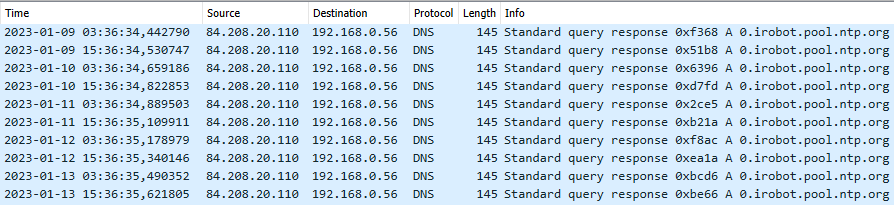
\includegraphics[width=\textwidth]{figures/NTP_wireshark .png}
    \caption{0.irobot.pool.ntp.org DNS resopnse}
    \label{fig:ntp_dns}
\end{figure}

\begin{figure}[H]
    \centering
    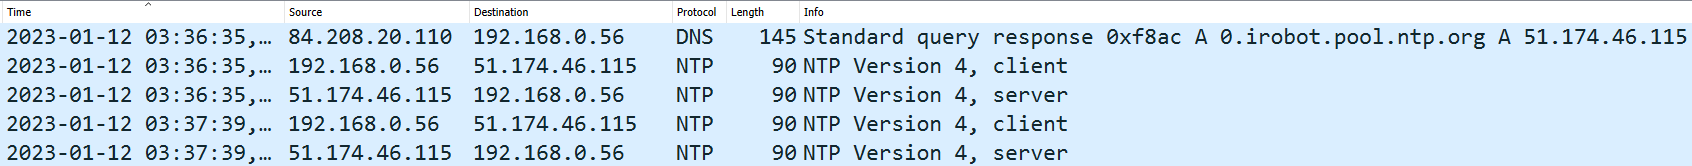
\includegraphics[width=\textwidth]{figures/ntp_dns.png}
    \caption{NTP and DNS realtion}
    \label{fig:ntp_dns2}
\end{figure}

\paragraph{DNS} is used by both the robot vacuum cleaner and the AP. The AP is using DNS request to determine if it is connected to Internet or not. This request is for a.root-servers.net, shown in \ref{fig:dns_a-root}.

\begin{figure}[H]
    \centering
    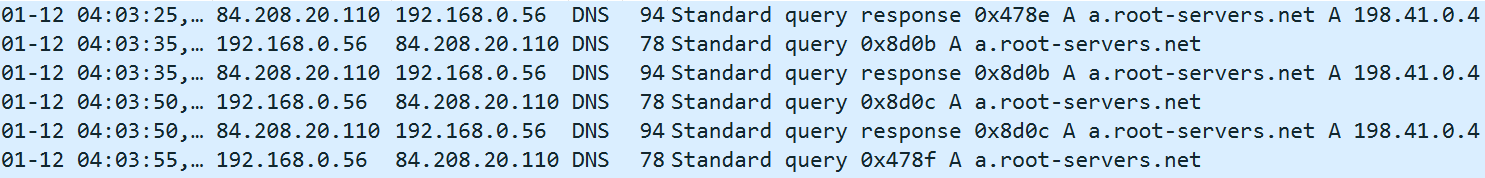
\includegraphics[width=\textwidth]{figures/DNS_a-root.png}
    \caption{Reoccurring DNS Internet test}
    \label{fig:dns_a-root}
\end{figure}

There is two more reocuring DNS reqests created from the TP-link access point. These are requested every three days, most likely to search for updates or upload statistics. DNS requests generated by the AP was therefore not included in further analysis, the different A records are listed below. 

\begin{itemize}
    \item a.rootservers.net
    \item n-devs-gw.tplinkcloud.com
    \item n-deventry-gw.tplinkcloud.com
\end{itemize}

The Irobot roomba requested the FQDNs listed below, once or tiwce a day. 
\begin{itemize}
    \item 0.irobot.pool.ntp.org
    \item disc-prod.iot.irobotapi.com
    \item unauth1.prod.iot.irobotapi.com
    \item a2uowfjvhio0fa.iot.us-east-1.amazonaws.com
\end{itemize}

After unauth1.prod.iot.irobotapi.com and disc-prod.iot.irobotapi.com, is requested there is a short traffic flow between the robot vacuum cleaner and the FQDNs. When these URLs was opened in a web-browser, we got prompted this message \textit{"message":"Missing Authentication Token"}. An authentication token was missing, and are probably exchanged when the Irobot Roomba establish the connection to the Irobot could service. 

a2uowfjvhio0fa.iot.us-east-1.amazonaws.com is requested once a day. When the robot vacuum cleaner receives the response it terminates the ongoing tcp session with the cloud control server, and establish a new one with one of the Ip addresses in the DNS response. Right after the establishment of the new control connection, a burst of traffic is sent between the Irobot and the could service. This is probably some information exchange to the new server. An attacker will have to eavesdrop the WAN connection of a smart environment, for maximum 24 hours to capture this DNS response. DNS traffic can therefore not be excluded, but used in identification of corresponding Irobot services. 

\subsection{TCP Traffic in standby traffic capture}
Continuous tcp traffic was sent between the Irobot Roomba and the Irobot could service. This is probably tcp-keep-alive traffic since these robots usually are located behind a WAN interface using NAT. The traffic therefore needs to be initiated from the vacuum cleaner. This traffic flow is shown in Figure \ref{fig:tcp_keep-alive}. The larges package sent in the tcp-keep-alive flow was 97 bytes, we assume that all packets with event data is more then 97 bytes. TCP packages less then 97 bytes was therefore excluded from further analysis. 

\begin{figure}[H]
    \centering
    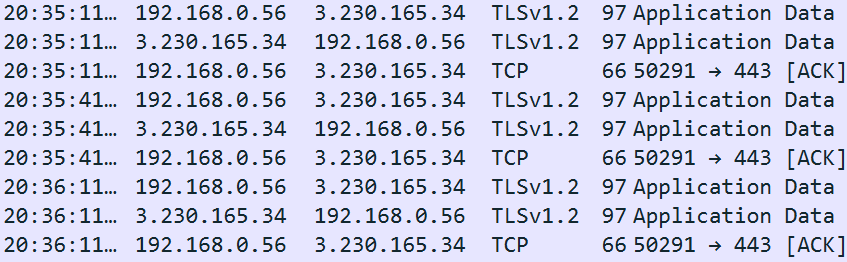
\includegraphics[width=\textwidth]{figures/tcp_keep-alive.png}
    \caption{Reoccurring DNS Internet test}
    \label{fig:tcp_keep-alive}
\end{figure}

\subsection{Base filter results}
The base filter was created based on the observations and conclusions from the overall section. DHCP, ARP and NTP traffic is excluded from further analysis. All packets less then 98 bytes was also excluded, this also excluded DNS traffic generated from the AP to test Internet connectivity. Used base filter was therefore; \textbf{!ntp \&\& !dhcp \&\& !arp \&\& frame.len > 97} \cite{wireshark}.

Larger DNS requests from the AP was still included in the capture, due to large packet size and identical packet length as some of the DNS request from the Irobot Roomba. When the base filter was applied on the standby traffic event, we successfully excluded 99,2\% of the captured traffic. This made the manual analysis more efficient. 

\section{Data Analysis}
In this section the entire analysis process for each individual event will be presented separately. In the last subsection there will be a summary and comparison on the different signatures identified.

\subsection{Data Analysis for Scheduled Cleaning}
The overall characteristics for this event is shown in Table \ref{tab:scoverall} and \ref{tab:scoverallDRA}. As presented the average and the standard deviation within the different environments are small. This supports the hypothesis that 20 events was sufficient.

\begin{table}[H]
\centering
\caption{Scheduled cleaning, overall statistics Oslo smart home}
\label{tab:scoverall}
\begin{tabular}{|l|l|l|}
\hline
\textbf{Event} & \textbf{Number of pkt} & \textbf{Total bytes sent} \\ \hline
Event 1        & 2541                   & 3669941                   \\ \hline
Event 2        & 2633                   & 3678959                   \\ \hline
Event 3        & 2622                   & 3660004                   \\ \hline
Event 4        & 2524                   & 3629262                   \\ \hline
Event 5        & 2627                   & 3658515                   \\ \hline
Event 6        & 2608                   & 3729110                   \\ \hline
Event 7        & 2596                   & 3645238                   \\ \hline
Event 8        & 2655                   & 3685536                   \\ \hline
Event 9        & 2573                   & 3713211                   \\ \hline
Event 10       & 2636                   & 3768883                   \\ \hline
Average        & 2601.5                 & 3683865.9                 \\ \hline
Standard deviation        & 43.03       & 42219,79               \\ \hline
\end{tabular}
\end{table}

\begin{table}[H]
\centering
\caption{Scheduled cleaning, overall statistics Drammen}
\label{tab:scoverallDRA}
\begin{tabular}{|l|l|l|}
\hline
\textbf{Event} & \textbf{Number of pkt} & \textbf{Total bytes sent} \\ \hline
Event 1        & 996                    & 1354755                   \\ \hline
Event 2        & 1052                   & 1422052                   \\ \hline
Event 3        & 1150                   & 1592566                   \\ \hline
Event 4        & 1317                   & 1650499                   \\ \hline
Event 5        & 1166                   & 1570805                   \\ \hline
Event 6        & 1179                   & 1612050                   \\ \hline
Event 7        & 1160                   & 1582275                   \\ \hline
Event 8        & 1177                   & 1610090                   \\ \hline
Event 9        & 1205                   & 1634883                   \\ \hline
Event 10       & 1170                   & 1590726                   \\ \hline
Average        & 1157.2                 & 1562070.1                 \\ \hline
Standard deviation        & 85,66
       & 95885,11               \\ \hline
\end{tabular}
\end{table}

In figure \ref{fig:Sc-graph}, the overall traffic flow is displayed. The traffic flow is consistence for all the captured scheduled cleaning events. The large spike of traffic is the session between the vacuum cleaner and S3.amasoneaws.com. There is also a increase in generated traffic at the start of the event, but this is 
deafened by the large upload traffic after finished cleaning.
\begin{figure}[H]
    \centering
    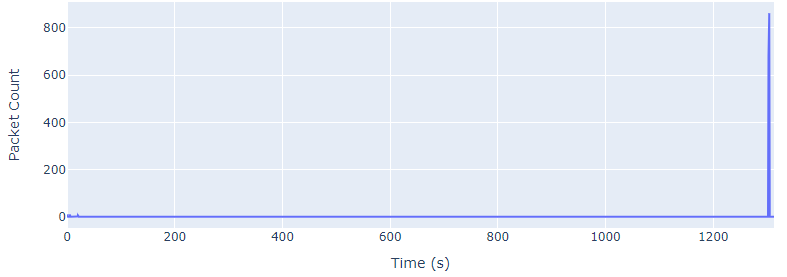
\includegraphics[width=\textwidth]{figures/SC-graph.png}
    \caption{Scheduled clean event 2}
    \label{fig:Sc-graph}
\end{figure}

\subsubsection{Protocol Identification}
In scheduled cleaning there is an average protocol distribution according to Table \ref{tab:scanalysisdist}, this after the base filter was applied. The two UDP packages is DNS response for FQDN:

\begin{itemize}
    \item 0550315.ingest.sentry.io
    \item S3.amasoneaws.com
\end{itemize}

\begin{table}[H]
\centering
\caption{Protocol Statistics Scheduled cleaning}
\label{tab:scanalysisdist}
\begin{tabular}{|c|c|}
\hline
\textbf{Transport protocol} & \textbf{Percentage} \\ \hline
UDP                         & 0,2                 \\ \hline
TCP                         & 99,8                \\ \hline
\end{tabular}
\end{table}

After a cleaning was done, there were two new sessions established. First a session to \textit{0550315.ingest.sentry.io} where the vacuum cleaner is transferring some data. Followed by a session to \textit{s3.amazoneaws.com}, where there is sent large amounts of traffic, before the session got terminated. Both sessions are established and teared down within a minute after a cleaning event was finished. This is most likely two different update services, where \textit{s3.amazoneaws.com} is the destination, for information about the cleaning and smart environment.
 
\subsubsection{Traffic Sequence}
All traffic had the WAN address as source or destination due to the infrastructure design. We extracted the first 20  packets in the traffic flow, to try to identify a common sequence for all Scheduled cleaning events. Only the first packets were examined, because that is where the event was triggered. In Figure \ref{fig:Scseq}, packet lengths of the 20 first packets are presented. The horizontal values are packet lengths, where notation 's' and 'd' are WAN address source or destination.  
For this event we could identified two packet sequences, they are listed below. The (+) or (-) indicated that all packet lengths can differ with the associated number. 

\begin{enumerate}
    \item \textit{[176, 173, 179, 443, 177]}, + - 15 bytes on all values 
    \item \textit{[176, 443, 179, 443, 177]} + - 5 bytes in all values
\end{enumerate}

\begin{figure}[H]
    \centering
    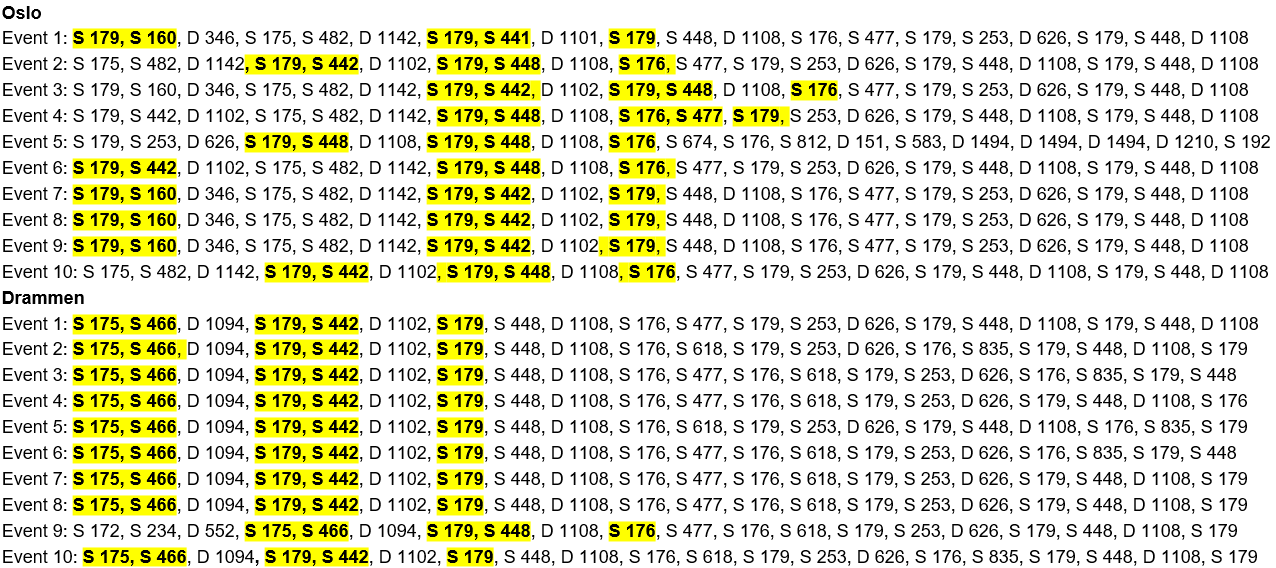
\includegraphics[width=\textwidth]{figures/Sequence_SC.png}
    \caption{Scheduled clean sequence}
    \label{fig:Scseq}
\end{figure}

\subsubsection{Signature}
The identified signature for Schedule cleaning includes the present of two DNS responses, and one of the given packet length sequences.  

\begin{itemize}
    \item \textit{0550315.ingest.sentry.io}
    \item \textit{s3.amazoneaws.com}
    \item \textit{[176, 173, 179, 443, 177]} +- 15
    \item \textit{[176, 443, 179, 443, 177]} +- 5
\end{itemize}

\subsection{Data Analysis for Automated Cleaning}
The overall characteristics for this event are shown in Table \ref{tab:scoverall} and \ref{tab:scoverallDRA}. As presented the average and the standard deviation within the different environments are small. This supports the hypothesis that 20 captures are sufficient. Event 6 in Drammen has a small amount of traffic compared to the other captures. During analysis, all identifications for a cleaning event was present, but the upload traffic towards S3.amazoneaws.com below average. This could be due to some disruption in the transaction or the lack of updates for the vacuum cleaner. 

\begin{table}[H]
\centering
\caption{Automated cleaning, overall statistics Oslo}
\label{tab:ACoverallOSL}
\begin{tabular}{|l|l|l|}
\hline
\textbf{Event} & \textbf{Packet number} & \textbf{Total bytes sent} \\ \hline
Event 1        & 2703                   & 3882164                   \\ \hline
Event 2        & 2736                   & 3811206                   \\ \hline
Event 3        & 2659                   & 3818287                   \\ \hline
Event 4        & 2681                   & 3747788                   \\ \hline
Event 5        & 2589                   & 3704329                   \\ \hline
Event 6        & 236                    & 237163                    \\ \hline
Event 7        & 2701                   & 3860634                   \\ \hline
Event 8        & 2631                   & 3770236                   \\ \hline
Event 9        & 2609                   & 3738406                   \\ \hline
Event 10       & 2609                   & 3799896                   \\ \hline
Average        & 2415.4                 & 3437010.9                 \\ \hline
Standard deviation        & 767.27
       & 1125643               \\ \hline
\end{tabular}
\end{table}

\begin{table}[H]
\centering
\caption{Overall statistics for Automated Cleaning in Drammen}
\label{tab:ACoverallDRA}
\begin{tabular}{|l|l|l|}
\hline
\textbf{Event} & \textbf{Packet number} & \textbf{Total bytes sent} \\ \hline
Event 1        & 1074                   & 1443851                   \\ \hline
Event 2        & 1131                   & 1524076                   \\ \hline
Event 3        & 1209                   & 1644223                   \\ \hline
Event 4        & 1207                   & 1641145                   \\ \hline
Event 5        & 1013                   & 1422457                   \\ \hline
Event 6        & 1013                   & 1422457                   \\ \hline
Event 7        & 1220                   & 1726862                   \\ \hline
Event 8        & 1248                   & 1715015                   \\ \hline
Event 9        & 1227                   & 1669154                   \\ \hline
Event 10       & 1456                   & 1838832                   \\ \hline
Average        & 1179.8                 & 1604807.2                 \\ \hline
Standard deviation        & 131.48
       & 144434.9               \\ \hline
\end{tabular}
\end{table}

In figure \ref{fig:Ac-graph}, the overall traffic flow is displayed. The traffic flow is consistence for all the captured events, and the large spike of traffic is the session between the vacuum cleaner and S3.amasoneaws.com. There is also a increase in generated traffic at the start of the event, but this is 
deafened by the large upload traffic after finished cleaning.

\begin{figure}[H]
    \centering
    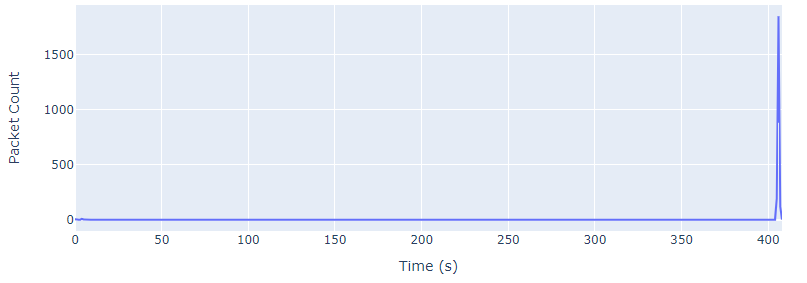
\includegraphics[width=\textwidth]{figures/AC-graph.png}
    \caption{Automated clean event 2 Oslo}
    \label{fig:Ac-graph}
\end{figure}

\subsubsection{Protocol Identification}
In Automated cleaning there is an average protocol distribution according to Table \ref{tab:acanalysisdist}. All the udp traffic is DNS requests, one to each of these FQDNs, listed below.

\begin{itemize}
    \item 0550315.ingest.sentry.io
    \item S3.amasoneaws.com
\end{itemize}

\begin{table}[H]
\centering
\caption{Protocol Statistics Automated cleaning}
\label{tab:acanalysisdist}
\begin{tabular}{|c|c|}
\hline
\textbf{Transport protocol} & \textbf{Percentage} \\ \hline
UDP                         & 0,1                 \\ \hline
TCP                         & 99,9                \\ \hline
\end{tabular}
\end{table}

After the cleaning was done, there is two new sessions established. First a session to \textit{0550315.ingest.sentry.io} where the vacuum cleaner is transferring some data. When this session is closed it opens a session to \textit{s3.amazoneaws.com}, where there is sent large amounts of traffic, before the session is closed. Both sessions are established and teared down within a minute after the cleaning is done. This is most likely two different update services where \textit{s3.amazoneaws.com} is where sensed information is uploaded and processed after cleaning.

\subsubsection{Traffic Sequence}
In all 20 events there is a common traffic sequence initiated from the could service, this is the packet length pair\textit{[316, 289]}. These packet lengths dose not occur in the same order, but is received together as a pair. So both \textit{[316, 289]} and \textit{[289, 315]} are valid. The actual packet length also varies with +- 1 byte. 
The following sequence is a response from the vacuum cleaner with packet lengths of \textit{[176, 187]}. Followed by a response from the cloud server with packet length 408 or 409. The identified sequence is therefore: \textit{[316, 289, 176, 187, 409]} or \textit{[289, 316, 176, 187, 409]} +- 1 byte.

\begin{figure}[H]
    \centering
    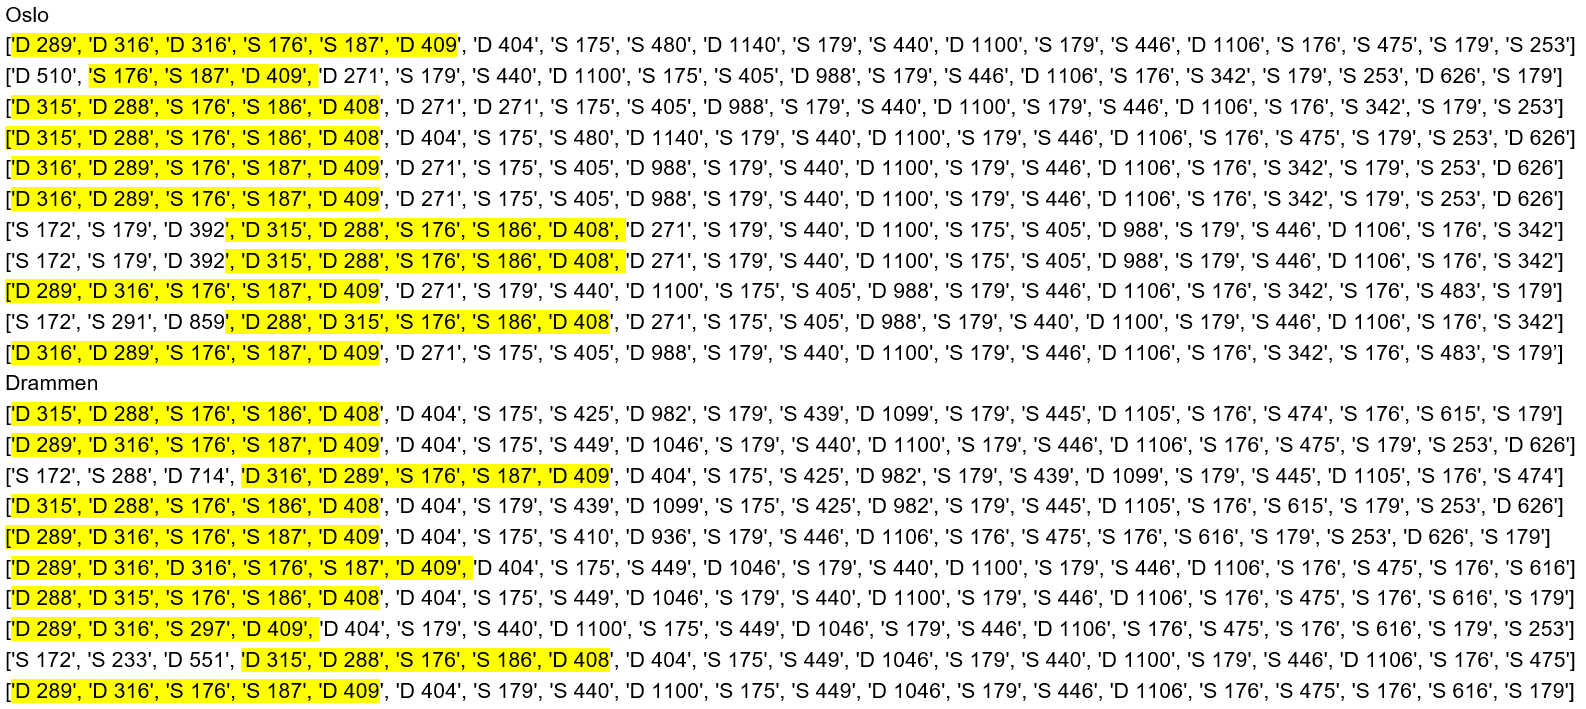
\includegraphics[width=\textwidth]{figures/Sequence_AC.png}
    \caption{Automated clean sequence}
    \label{fig:ACseq}
\end{figure}


\subsubsection{Signature}
The identified signature for Automated cleaning includes the presents of two DNS responses and one of the given sequences, listed below.  

\begin{itemize}
    \item \textit{0550315.ingest.sentry.io}
    \item \textit{s3.amazoneaws.com}
    \item \textit{[316, 289, 176, 187, 409]} +- 1
    \item \textit{[289, 316, 176, 187, 409]} +- 1
\end{itemize}


\subsection{Data Analysis for Application Triggered Cleaning}
The overall characteristics for this event is presented in Table \ref{tab:TCoverallOSL} and \ref{tab:TCoverallDRA}. As presented the average and the standard deviation within the different environments is small. This supports the hypothesis that is is sufficient with 20 captured events to perform further analysis.

\begin{table}[H]
\centering
\caption{Application triggered cleaning, overall statistics Oslo}
\label{tab:TCoverallOSL}
\begin{tabular}{|l|l|l|}
\hline
\textbf{Event} & \textbf{Packet number} & \textbf{Total bytes sent} \\ \hline
Event 1        & 2667                   & 3732218                   \\ \hline
Event 2        & 2686                   & 3730748                   \\ \hline
Event 3        & 2656                   & 3710958                   \\ \hline
Event 4        & 3065                   & 4365510                   \\ \hline
Event 5        & 2880                   & 4076534                   \\ \hline
Event 6        & 2633                   & 3771269                   \\ \hline
Event 7        & 2661                   & 3786648                   \\ \hline
Event 8        & 2647                   & 3798184                   \\ \hline
Event 9        & 2729                   & 3798630                   \\ \hline
Event 10       & 2639                   & 3786194                   \\ \hline
Average        & 2726.3                 & 3855689.3                 \\ \hline
Standard deviation        & 139.57
       & 206499.4               \\ \hline
\end{tabular}
\end{table}

\begin{table}[H]
\centering
\caption{Application triggered cleaning, overall statistics Drammen}
\label{tab:TCoverallDRA}
\begin{tabular}{|l|l|l|}
\hline
\textbf{Event} & \textbf{Packet number} & \textbf{Total bytes sent} \\ \hline
Event 1        & 708                    & 802488                    \\ \hline
Event 2        & 724                    & 945100                    \\ \hline
Event 3        & 740                    & 956470                    \\ \hline
Event 4        & 809                    & 1071613                   \\ \hline
Event 5        & 824                    & 1088836                   \\ \hline
Event 6        & 869                    & 1157323                   \\ \hline
Event 7        & 855                    & 1144086                   \\ \hline
Event 8        & 929                    & 1248783                   \\ \hline
Event 9        & 988                    & 1321061                   \\ \hline
Event 10       & 983                    & 1339631                   \\ \hline
Average        & 842.9                  & 1107539.1                 \\ \hline
Standard deviation        & 101.85
       & 172281.2               \\ \hline
\end{tabular}
\end{table}

In figure \ref{fig:Tc-graph}, the overall traffic flow is displayed. The traffic flow is consistence for all the captured events, and the large spike of traffic is the session between the vacuum cleaner and S3.amasoneaws.com. There is also a increase in generated traffic at the start of the event, but this is 
deafened by the large upload traffic after finished cleaning.

\begin{figure}[H]
    \centering
    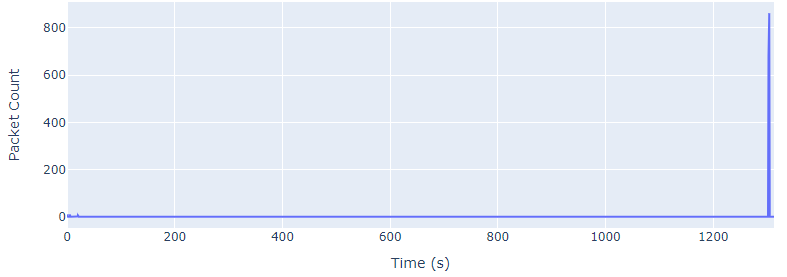
\includegraphics[width=\textwidth]{figures/TC-graph.png}
    \caption{Application triggered clean event 2, Oslo}
    \label{fig:Tc-graph}
\end{figure}

\subsubsection{Protocol Identification}
In Automated cleaning there is an average protocol distribution according to \ref{tab:tcanalysisdist}. All the udp traffic is DNS request, one to each of these FQDNs:

\begin{table}[H]
\centering
\caption{Protocol Statistics Application Triggered Cleaning}
\label{tab:tcanalysisdist}
\begin{tabular}{|c|c|}
\hline
\textbf{Transport protocol} & \textbf{Percentage} \\ \hline
UDP                         & 0,1                 \\ \hline
TCP                         & 99,9                \\ \hline
\end{tabular}
\end{table}



After the cleaning is done, there is two new sessions established. First a session to \textit{0550315.ingest.sentry.io} where the vacuum cleaner is transferring some data. When this session is closed it opens a session to \textit{s3.amazoneaws.com}, where there is sent large amounts of traffic, before the session is closed. Both sessions are established and teared down within a minute after the cleaning is done. This is most likely two different update services where \textit{s3.amazoneaws.com} is where sensed information is uploaded and processed after cleaning.

\subsubsection{Traffic Sequence}
All events has a common sequence initiated from the cloud service, \textit{[209, 289, 316]}. The two last packets can be in mixed order. A response from the vacuum cleaner with two packets of lengths \textit{176, 187} is then sent. This is followed by a response from the could service with a package of length \textit{409 or 408}. The entire packet sequences are then \textit{[316, 289, 176, 187, 409] or [289, 316, 176, 187, 409]
}

\begin{figure}[H]
    \centering
    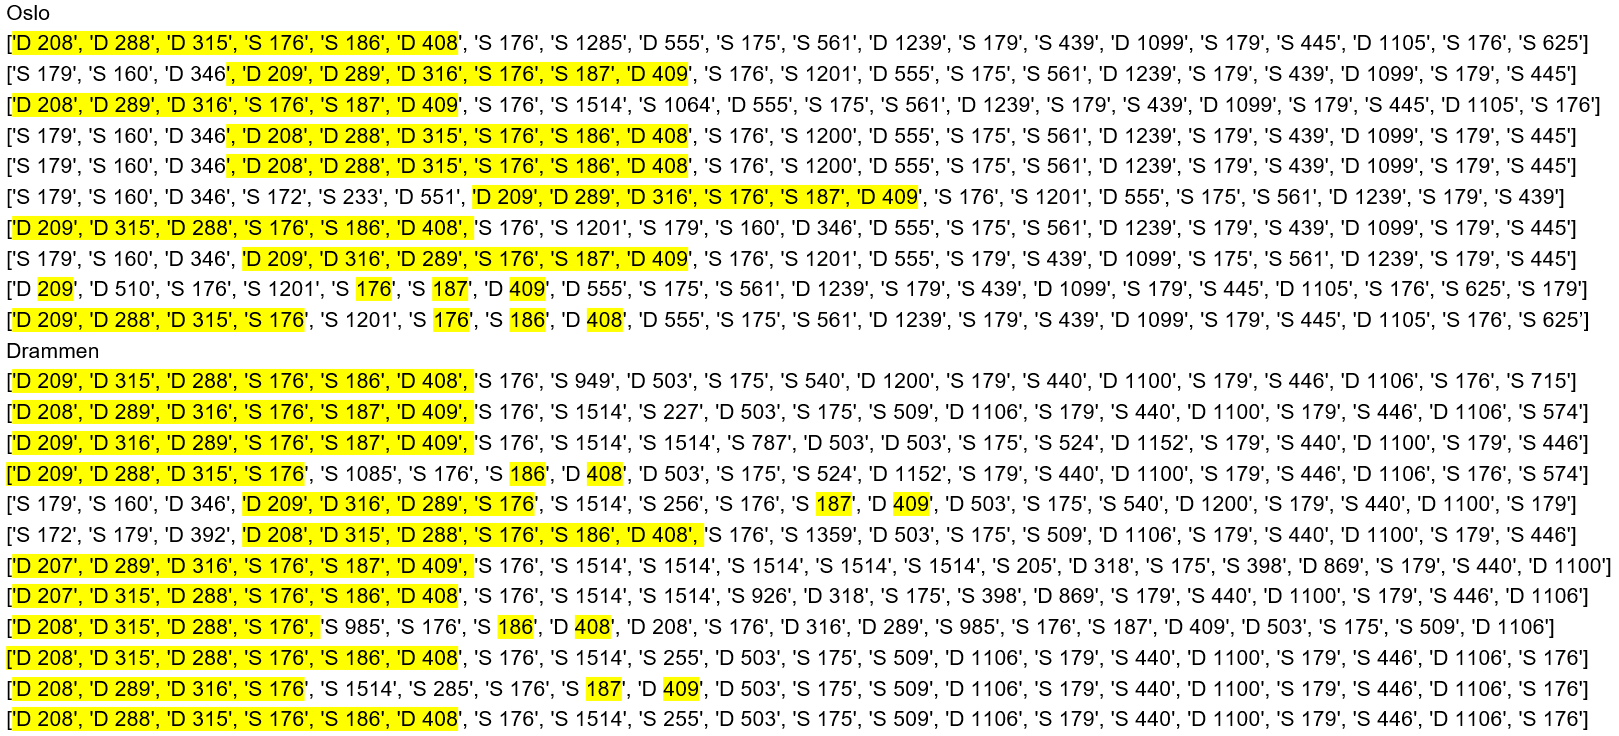
\includegraphics[width=\textwidth]{figures/Sequence_ATC.png}
    \caption{Application triggered cleaning sequence}
    \label{fig:ATCseq}
\end{figure}

\subsubsection{Signature}
The identified signature for Application triggered cleaning includes the present of two DNS responses and one of the given sequences, listed below.
\begin{itemize}
    \item 0550315.ingest.sentry.io
    \item s3.amazoneaws.com
    \item \textit{[209, 316, 289, 176, 187, 409] +- 1}
    \item \textit{[209, 289, 316, 176, 187, 409] +- 1}
\end{itemize}

\subsection{Data Analysis for Physical Triggered Cleaning}
The overall characteristics for this event is shown in table \ref{tab:PCoverallOSL} and \ref{tab:PCoverallDRA}. As presented the average and the standard deviation within the different environments is small. This supports the hypothesis that it is sufficient with 20 captured events to perform further analysis.
\begin{table}[H]
\centering
\caption{Physical triggered cleaning, overall statistics Oslo}
\label{tab:PCoverallOSL}
\begin{tabular}{|l|l|l|}
\hline
\textbf{Event} & \textbf{Packet number} & \textbf{Total bytes sent} \\ \hline
Event 1        & 2791                   & 3965147                   \\ \hline
Event 2        & 3180                   & 4357126                   \\ \hline
Event 3        & 2926                   & 4033946                   \\ \hline
Event 4        & 2872                   & 4112516                   \\ \hline
Event 5        & 2944                   & 4209443                   \\ \hline
Event 6        & 2984                   & 4122412                   \\ \hline
Event 7        & 2925                   & 4160462                   \\ \hline
Event 8        & 2869                   & 4100166                   \\ \hline
Event 9        & 2918                   & 4227626                   \\ \hline
Event 10       & 2768                   & 3957559                   \\ \hline
Average        & 2917.7                 & 4124640.3                 \\ \hline
Standard deviation        & 113.98
       & 122683.4               \\ \hline
\end{tabular}
\end{table}

\begin{table}[H]
\centering
\caption{Physical triggered cleaning, overall statistics Drammen}
\label{tab:PCoverallDRA}
\begin{tabular}{|l|l|l|}
\hline
\textbf{Event} & \textbf{Packet number} & \textbf{Total bytes sent} \\ \hline
Event 1        & 1078                   & 1481677                   \\ \hline
Event 2        & 1087                   & 1484930                   \\ \hline
Event 3        & 1125                   & 1520872                   \\ \hline
Event 4        & 1088                   & 1517429                   \\ \hline
Event 5        & 1150                   & 1555605                   \\ \hline
Event 6        & 1086                   & 1507084                   \\ \hline
Event 7        & 1092                   & 1501894                   \\ \hline
Event 8        & 1115                   & 1510971                   \\ \hline
Event 9        & 1098                   & 1485863                   \\ \hline
Event 10       & 1100                   & 1492331                   \\ \hline
Average        & 1101.9                 & 1505865.6                 \\ \hline
Standard deviation        &22.05
       & 22318.19               \\ \hline
\end{tabular}
\end{table}

In figure \ref{fig:Pc-graph}, the overall traffic flow is displayed. The traffic flow is consistence for all the captured events, and the large spike of traffic is the session between the vacuum cleaner and S3.amasoneaws.com. There is also a increase in generated traffic at the start of the event, but this is 
deafened by the large upload traffic after finished cleaning.
\begin{figure}[H]
    \centering
    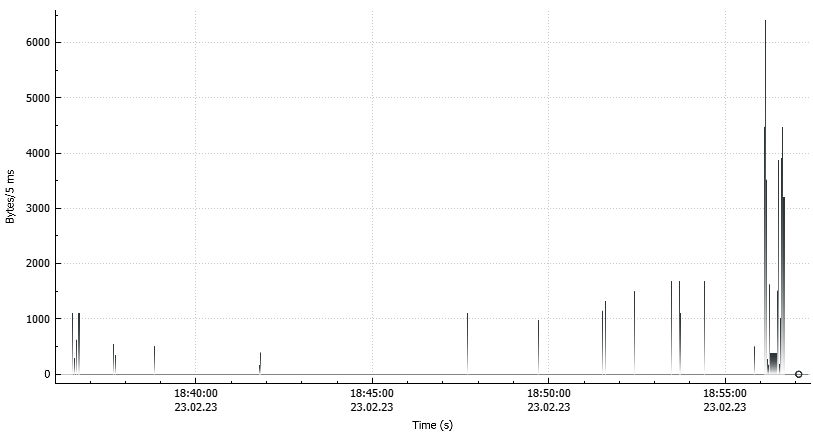
\includegraphics[width=\textwidth]{figures/PC-graph.png}
    \caption{Physical cleaning}
    \label{fig:Pc-graph}
\end{figure}

\subsubsection{Protocol Identification}
In Automated cleaning there is an average protocol distribution according to \ref{tab:pcanalysisdist}. All the udp traffic is DNS request, one to each of these FQDNs

\begin{table}[H]
\centering
\caption{Protocol statistics physical triggered cleaning}
\label{tab:pcanalysisdist}
\begin{tabular}{|c|c|}
\hline
\textbf{Transport protocol} & \textbf{Percentage} \\ \hline
UDP                         & 0,1                 \\ \hline
TCP                         & 99,9                \\ \hline
\end{tabular}
\end{table}

After the cleaning is done, there is two new sessions established. First a session to \textit{0550315.ingest.sentry.io} where the vacuum cleaner is transferring some data. When this session is closed it opens a session to \textit{s3.amazoneaws.com}, where there is sent large amounts of traffic, before the session is closed. Both sessions are established and teared down within a minute after the cleaning is done. This is most likely two different update services where \textit{s3.amazoneaws.com} is where sensed information is uploaded and processed after cleaning.

\subsubsection{Traffic Sequence}
 Packet lengths for the first 20 packets are presented in Figure \ref{fig:PCseq}. There is no initial traffic sequence to identify in this event, but there is a reoccurring pattern where the vacuum cleaner sends packets with the length of \textit{[176, 173, 179, 443, 177]} or \textit{[176, 443, 179, 443, 177]}. This traffic flow is continuing throughout the duration of the cleaning. The identified sequence is listed below.
\begin{itemize}
    \item \textit{[176, 173, 179, 443, 177]}, + - 15 bytes on all values 
    \item \textit{[176, 443, 179, 443, 177]} + - 5 bytes in all values
\end{itemize}

The reason for adding + or - 15 and 5 is because the actual value is varies with the deviation of 15 and 5.

\begin{figure}[H]
    \centering
    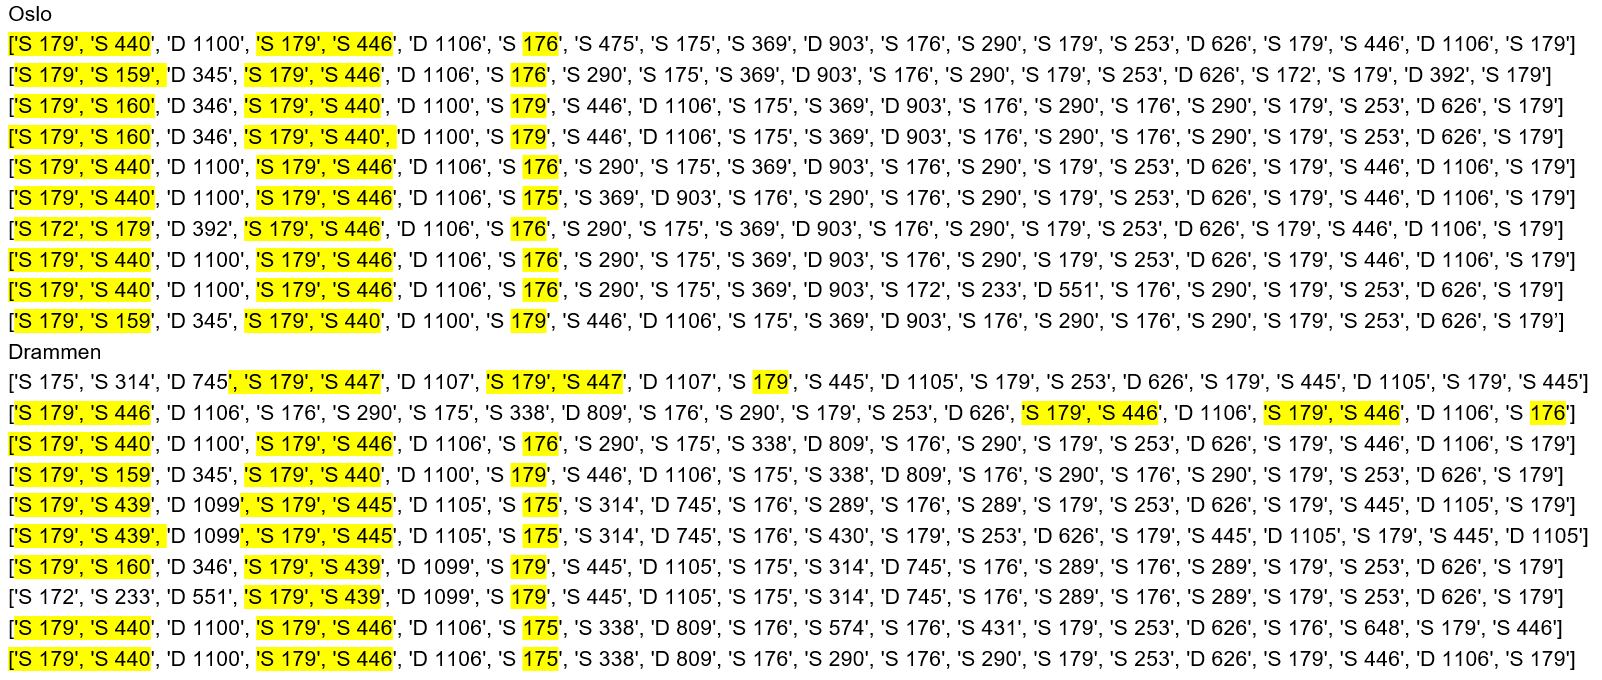
\includegraphics[width=\textwidth]{figures/Sequence_PC.png}
    \caption{Physical triggered cleaning sequences}
    \label{fig:PCseq}
\end{figure}

\subsubsection{Signature}
The identified signature for Physical triggered cleaning includes the present of two DNS responses and one of the given sequences.  

\begin{itemize}
    \item \textit{0550315.ingest.sentry.io}
    \item \textit{s3.amazoneaws.com}
    \item \textit{[176, 173, 179, 443, 177]} +- 15
    \item \textit{[176, 443, 179, 443, 177]} +- 5
\end{itemize}

\subsection{Data Analysis for Application Start}
The captures including Application start event has a small amount of network traffic. The deviation is therefore large, but the difference in in how long the application was open and actions, could cause this variation. In Drammen, event 5 to 10 was used to change the time for a scheduled cleaning event. This can be identified in table \ref{tab:TestMatrixEnv2}, as more traffic is generated. The same procedure should have been followed to create more stable results. This research will therefor only focus on the initial traffic flow.

\begin{table}[H]
\centering
\caption{Application start, overall statistics Oslo}
\label{tab:ASoverallOslo}
\begin{tabular}{|l|l|l|}
\hline
\textbf{Event} & \textbf{Packet number} & \textbf{Total bytes sent} \\ \hline
Event 1        & 11                     & 5202                      \\ \hline
Event 2        & 22                     & 8698                      \\ \hline
Event 3        & 20                     & 8644                      \\ \hline
Event 4        & 17                     & 7135                      \\ \hline
Event 5        & 20                     & 8580                      \\ \hline
Event 6        & 20                     & 8608                      \\ \hline
Event 7        & 20                     & 9213                      \\ \hline
Event 8        & 23                     & 9527                      \\ \hline
Event 9        & 20                     & 8730                      \\ \hline
Event 10       & 19                     & 8877                      \\ \hline
Average        & 19.2                   & 8321.4                    \\ \hline
Standard deviation        & 3.29
       & 1258.62               \\ \hline
\end{tabular}
\end{table}

\begin{table}[H]
\centering
\caption{Application start, overall statistics Drammen}
\label{tab:ASoverallDRA}
\begin{tabular}{|l|l|l|}
\hline
\textbf{Event} & \textbf{Packet number} & \textbf{Total bytes sent} \\ \hline
Event 1        & 30                     & 20875                     \\ \hline
Event 2        & 26                     & 19568                     \\ \hline
Event 3        & 8                      & 2655                      \\ \hline
Event 4        & 8                      & 2659                      \\ \hline
Event 5        & 26                     & 19561                     \\ \hline
Event 6        & 34                     & 21897                     \\ \hline
Event 7        & 29                     & 20222                     \\ \hline
Event 8        & 25                     & 19468                     \\ \hline
Event 9        & 33                     & 21744                     \\ \hline
Event 10       & 26                     & 19570                     \\ \hline
Average        & 24,5                   & 16821.9                   \\ \hline
Standard deviation        & 9.22
       & 7519.30               \\ \hline
\end{tabular}
\end{table}

\subsubsection{Protocol Identification}
During an application start there is only tcp packages sent between the vacuum cleaner and the cloud service.

\subsubsection{Traffic Sequence}
All events has a common sequence initiated from the cloud service, \textit{[209, 289, 316]} where the two last packets can be in mixed order. The vacuum cleaner then responds with two packets with lengths of \textit{176, 187}, before the could service responds with a package with a length of \textit{409 or 408}. The entire packet sequence is then \textit{[316, 289, 176, 187, 409] or [289, 316, 176, 187, 409]}. This is identified in figure \ref{fig:ASseq}.

\begin{figure}[H]
    \centering
    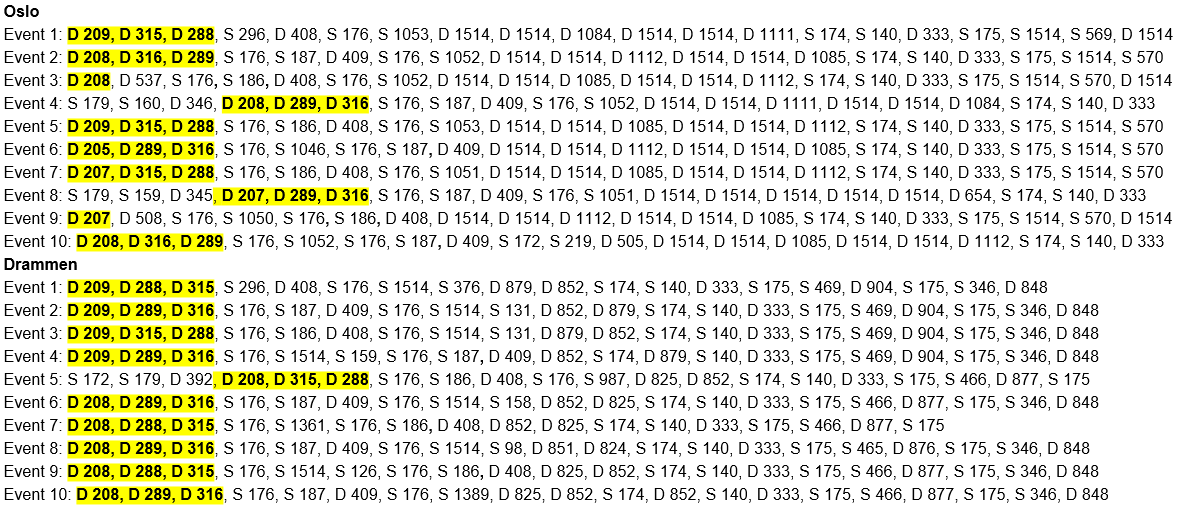
\includegraphics[width=\textwidth]{figures/Sequence_AS.png}
    \caption{Application start sequence}
    \label{fig:ASseq}
\end{figure}

\subsubsection{Signature}
The identified signature for Application start includes one of the given sequences.
\begin{itemize}
    \item \textit{[209, 316, 289, 176, 187, 409] +- 1}
    \item \textit{[209, 289, 316, 176, 187, 409] +- 1}
\end{itemize}


\subsection{Data Analysis for Bin Remove}
For the Bin remove event there is some deviations in traffic amount. Observations during the event triggering was, that sometimes the vacuum cleaner made a sound, sometimes it started flashing. This is probably because it lost connection with one of the charging connectors. This causes the event to be non standard and loose validity. The event will throughout this research be Bin remove, but it can be discussed if the event should be excluded.

\begin{table}[H]
\centering
\caption{Bin remove, overall statistics Oslo}
\label{tab:BRoverallOslo}
\begin{tabular}{|l|l|l|}
\hline
\textbf{Event} & \textbf{Packet number} & \textbf{Total bytes sent} \\ \hline
Event 1        & 6                      & 2512                      \\ \hline
Event 2        & 15                     & 5765                      \\ \hline
Event 3        & 12                     & 4366                      \\ \hline
Event 4        & 15                     & 7869                      \\ \hline
Event 5        & 12                     & 5022                      \\ \hline
Event 6        & 17                     & 8426                      \\ \hline
Event 7        & 18                     & 8492                      \\ \hline
Event 8        & 12                     & 5022                      \\ \hline
Event 9        & 11                     & 4956                      \\ \hline
Event 10       & 12                     & 5022                      \\ \hline
Average        & 13                     & 5745.2                    \\ \hline
Standard deviation        & 3.43
       & 1937.64               \\ \hline
\end{tabular}
\end{table}


\begin{table}[H]
\centering
\caption{Bin remove, overall statistics Drammen }
\label{tab:BRoverallDRA}
\begin{tabular}{|l|l|l|}
\hline
\textbf{Event} & \textbf{Packet number} & \textbf{Total bytes sent} \\ \hline
Event 1        & 23                     & 8610                      \\ \hline
Event 2        & 24                     & 10149                     \\ \hline
Event 3        & 9                      & 4407                      \\ \hline
Event 4        & 12                     & 5022                      \\ \hline
Event 5        & 8                      & 4333                      \\ \hline
Event 6        & 9                      & 4399                      \\ \hline
Event 7        & 17                     & 6595                      \\ \hline
Event 8        & 9                      & 4399                      \\ \hline
Event 9        & 15                     & 7869                      \\ \hline
Event 10       & 12                     & 5022                      \\ \hline
Average        & 13,8                   & 6080.5                    \\ \hline
Standard deviation        & 5.87
       & 2112.52               \\ \hline
\end{tabular}
\end{table}

\subsubsection{Protocol Identification}
During the event it is only captured TCP packages, since the number of packages is limited and the traffic is end-to-end encrypted with TLS there is not much information to extract. 

\subsubsection{Traffic Sequence}
The traffic sequence has to distinct packet lengths which is not identified in any og the previous events. This is \textit{410 and 411}, these packets are always received after the vacuum cleaner has sent two packets with the length of \textit{[179, 186]}. The distinct pattern is therefore \textit{[179, 187, 410]}

\begin{figure}[H]
    \centering
    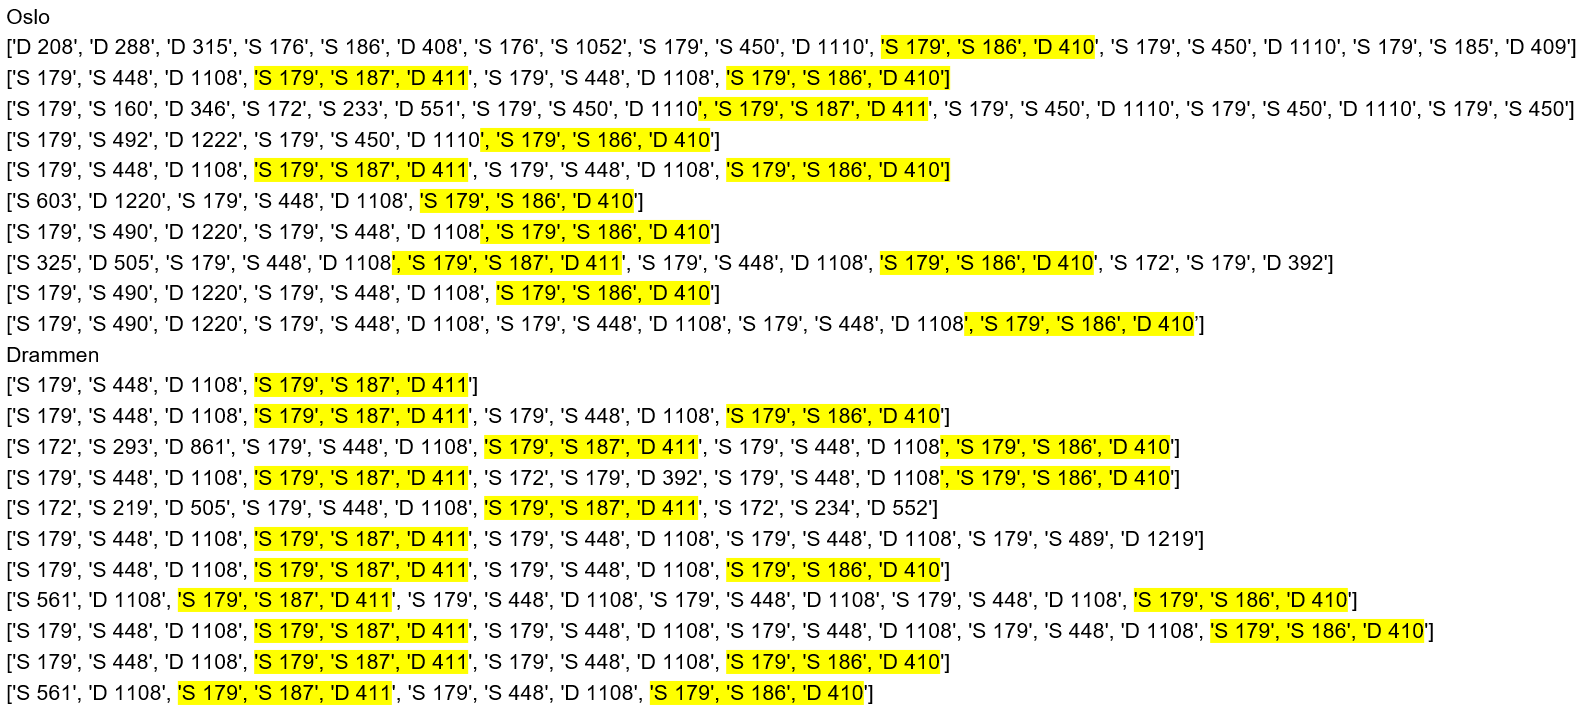
\includegraphics[width=\textwidth]{figures/Sequence_BR.png}
    \caption{Bin remove sequence}
    \label{fig:BRseq}
\end{figure}

\subsubsection{Signature}
The signature for Bin removal event is therefor the identification of this sequence
\begin{itemize}
    \item \textit{[179, 187, 410]} + - 1
\end{itemize}


\subsection{WLAN and LAN Analysis}
WLAN and LAN traffic were captured for all triggered events, but due to the thesis' time constrains we only identified signatures and detection algorithms on LAN captures. The simulated WAN traffic had more available attributes, due to the WiFI's encryption. \cite{pingpong_trimananda2020packet} have already proposed a method to identify actions based on packet lengths. We therefore focused on the WAN traffic, to be able to include DNS as a identifier. To evaluate if the same method and algorithm is applicable  to WLAN traffic we did a comparison of two corresponding captures. Through analysis we identified that the added WiFI header was 79 bytes, the base filter of 97 bytes in LAN captures was therefore converted to 176 bytes in WLAN. When this filter was applied we could identify the same packet sequences as in the simulated WAN traffic. These findings are presented in Figure \ref{fig:WLANLANHeader}. With the base filter applied we also observed that the WLAN capture included less packets then the corresponding LAN capture. This could be the result of retransmission, dual WiFi channels, signal disruption and packet collision on the NIC in monitoring mode. When the NIC was configured in monitoring mode, it collected all WiFi traffic in the area. This includes traffic from other SSIDs within wireless coverage. The original ISP modem, was also brocasting it's SSIDs, causing high Signal to Noise Ratio (SNR) for more then one SSID. Without control traffic between the AP and the NIC it could potentially lose traffic. Regardless of the packet loss we are still able to identify similar patterns in WLAN traffic. 

\begin{figure}[H]
    \centering
    \begin{subfigure}[b]{0.9\textwidth}
        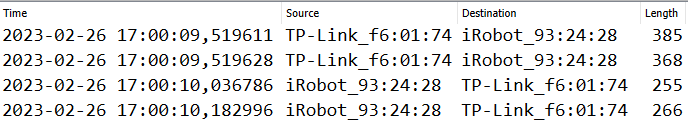
\includegraphics[width=\textwidth]{figures/WLANLANComparison.png}
        \caption{WLAN}
    \end{subfigure}
    \quad
    \begin{subfigure}[b]{0.9\textwidth}
        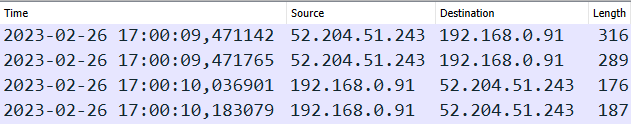
\includegraphics[width=\textwidth]{figures/LANWLANcomparison.png}
        \caption{LAN}
    \end{subfigure}
    
    \caption{WLAN and LAN comparison}
    \label{fig:WLANLANHeader}
\end{figure}

WLAN captures need more analysis before they can be implemented in the detection algorithm. An advantage of WLAN traffic is the availability of MAC addresses, an attacker can therefore easily identify the robot vacuum cleaner and filter traffic based on this information. Compared to LAN where an attackers will not have to eavesdrop for up to 24 hours, before the Irobot traffic can be identified. 
 

\subsection{Signature Comparison}
All the different cleaning events had the same DNS responses present in the packet capturing. First a DNS response for \textit{0550315.ingest.sentry.io}, followed by \textit{0550315.ingest.sentry.io}. These dns packets can therefore not be used as signature for any of the specific cleaning events, but as a confident test to identify that a cleaning is executed. There is several similarities between the identified sequences and this will be discussed further.

\paragraph{Comparison between Scheduled cleaning and Physical triggered cleaning event.} Both events had the identified packet length sequences listed below. 
\begin{itemize}
    \item \textit{[176, 173, 179, 443, 177]} +- 15
    \item \textit{[176, 443, 179, 443, 177]} +- 5
\end{itemize}
These sequences can therefore not differentiate the events. However the traffic sequence on all the scheduled cleaning events is started within a minute before the scheduled cleaning's configured trigger time. It is safe to assume that scheduled cleaning is configured every hole hour or half hour. A normal user would probably not configure a cleaning at 15:17, but at 15:00. If an attacker is monitoring a smart environment during a longer time period, the two different cleanings can be separated based on reoccurring identification. A identified cleaning every Monday at 07:59 is most likely a scheduled cleaning, since humans are not provide the same level of consistency.


\paragraph{Application start and Application Triggered Cleaning}
both event had the same identified sequence
\begin{itemize}
    \item \textit{[209, 316, 289, 176, 187, 409] +- 1}
    \item \textit{[209, 289, 316, 176, 187, 409] +- 1}
\end{itemize}
We can assume that this sequence is due to the fact that the application is started, and not the actual triggering of the cleaning event. It is still possible to differentiate between these two events with the use of Application triggered cleaning's DNS signature. As all other cleaning events it includes \textit{0550315.ingest.sentry.io} and then \textit{s3.amazoneaws.com}. If the application start sequences and the cleaning DNS responses is detected we can assume that a application triggered cleaning is executed. An element of uncertainty occurs if the user opens the application before or during another cleaning event, then this could create a false positive. 

\paragraph{Automated cleaning compared to Application triggered cleaning}
The only difference between these two events is the first package in Application start sequence. This packet has the length of 209 bytes and occurs 100 \% of the times the application is started. The identification of this is therefor a good attribute to differentiate for these events.

\section{Event Identification}
This section, presents logical sudo code  for all identification algorithms created through the analysis. Each algorithm aims to identify the presents of one signature. The raw python could is presented in Appendix \ref{app:DetectionAlgorithm}. 

\paragraph{Application start detection} will be used for both Application start and Application triggered cleaning detection. Sudo code is presented below.

\begin{figure}[H]
    \centering
    \caption{The algorithm for identifying the application-start event}
    \label{fig:Sudo_code_application start}
    \begin{lstlisting}[numbers=left]
     function detect_application_start(packet_lengths)
          signature1 = [209,289,316]
          signature2 = [209.316.289]
          if signature1 in packet_lengths
               application_start_confidence = + 10
          elsif signature1 in packet_lengths
              application_start_confidence = + 10
          return application_start_confidence
    \end{lstlisting}
\end{figure}

\paragraph{Cleaning detection} is done as a attribute to be used to add confidence to a cleaning event. 
\begin{figure}[H]
    \centering
    \caption{The algorithm for identifying general cleaning event}
    \label{fig:Sudo_code_cleaning_event}
    \begin{lstlisting}[numbers=left]
     function cleaning_event_detection(event_capture)
          if 'o550315.ingest.sentry.io' in event_capture
               dns1 == True
          elsif
               dns1 == False
          if 's3.amazonaws.com' in event_capture
               dns2 == True
          elsif
               dns2 == False
          if dns1 and dns2 == True      
               cleaning_confidece = + 10
          return cleaning_confident
    \end{lstlisting}
\end{figure}

\paragraph{Application triggered cleaning} is detected with a combination of Application start and cleaning detection.


\begin{figure}[H]
    \centering
    \caption{The algorithm for identifying the physical-triggered-cleaning-event}
    \label{fig:Sudo_code_application_triggered_cleaning_detection}
    \begin{lstlisting}[numbers=left]
     function application_triggered_cleaning(cleaning_confident, application_start_confident)
          if cleaning_confident and application_start_confident > 0
              application_triggered_cleaning_confident = + 10
          return application_triggered_cleaning_confident
    \end{lstlisting}
\end{figure}

\paragraph{Scheduled cleaning and Physical triggered cleaning}, time detection has not been implemented due to time limitations, but the sudo code for the detection based on the sequence is presented in the analysis. 


\begin{figure}[H]
    \centering
    \caption{Sudo code for scheduled or physical triggered cleaning detection}
    \label{fig:Sudo_code_SC_or_PC}
    \begin{lstlisting}[numbers=left]
     function detect_application_start(packet_lengths_src)
          signature1 = [176,173,179,443,177]
          signature2 = = [176,443,179,443,177]
          if signature1 in packet_lengths
               SC_PTC_confident = + 10
          elsif signature1 in packet_lengths
               SC_PTC_confident = + 10
          return SC_PTC_confident
    \end{lstlisting}
\end{figure}

\paragraph{Automated cleaning}, is identified as with the sequence identified in the analysis. 


\begin{figure}[H]
    \centering
    \caption{The algorithm for identifying the automated-cleaning event}
    \label{fig:Sudo_code_AC}
    \begin{lstlisting}[numbers=left]
     function detect_application_start(packet_lengths_src)
          signature1 = [316, 289, 176, 187, 409]
          signature2 = [289, 316, 176, 187, 409]
          if signature1 in packet_lengths
               automanted_cleaning_confident = + 10
          elsif signature1 in packet_lengths
               automated_cleaning_confident = + 10
    \end{lstlisting}
\end{figure}

